\chapter{Benchmark Models and Reference Results}
\label{chap:benchmarks}

%%%%%%%%%%%%%%%%%%%%%%%%%%%%%%%%%%%%%%%%%%%%%%%%%%%%%%%%%%%%%%%%%%%%%%%%%%%%%%%
\section{Motivation}
\label{sec:chap7-motivate}

\begin{itemize}[noitemsep]
  \item identify metrics of interest - eigenvalue, fission, capture rates
  \item match CE MC as closely as possible with deterministic MG theory
  \item understand spatial self-shielding effects in pin-wise MGXS
\end{itemize}


%%%%%%%%%%%%%%%%%%%%%%%%%%%%%%%%%%%%%%%%%%%%%%%%%%%%%%%%%%%%%%%%%%%%%%%%%%%%%%%
\section{Benchmark Configurations}
\label{sec:chap7-benchmarks}

\begin{table}[h!]
  \centering
  \caption[BEAVRS isotopic composition]{BEAVRS isotopic composition.}
  \tiny
  \label{table:chap7-beavrs-isotopes} 
  \vspace{6pt}
  \begin{tabular}{c c}
  \toprule
  \rowcolor{lightgray}
  {\bf Nuclide} &
  {\bf Density [atom/b-cm]} \\
  \midrule
  \multicolumn{2}{c}{\bf Air (0.000616 g/cc)} \\
  \midrule
  C-12 & 6.7565e-09 \\
  C-13 & 7.3076e-11 \\
  O-16 & 5.2864e-06 \\
  O-17 & 2.0137e-09 \\
  N-14 & 1.9681e-05 \\
  N-15 & 7.1900e-08 \\
  Ar-36 & 7.9414e-10 \\
  Ar-38 & 1.4915e-10 \\
  Ar-40 & 2.3506e-07 \\
  \midrule
  \multicolumn{2}{c}{\bf Borated Water (0.740582 g/cc)} \\
  \midrule
  H-1 & 4.9457e-02 \\
  H-2 & 7.4196e-06 \\
  B-10 & 8.0042e-06 \\
  B-11 & 3.2218e-05 \\
  O-16 & 2.4672e-02 \\
  O-17 & 9.3982e-06 \\
  \midrule
  \multicolumn{2}{c}{\bf Borosilicate Glass (2.260000 g/cc)} \\
  \midrule
  B-10 & 9.6506e-04 \\
  B-11 & 3.9189e-03 \\
  O-16 & 4.6511e-02 \\
  O-17 & 1.7717e-05 \\
  Al-27 & 1.7352e-03 \\
  Si-28 & 1.6924e-02 \\
  Si-29 & 8.5977e-04 \\
  Si-30 & 5.6743e-04 \\
  \midrule
  \multicolumn{2}{c}{\bf 1.6\% Enriched UO$_2$ (10.31341 g/cc)} \\
  \midrule
  U-234 & 3.0131E-06 \\
  U-235 & 3.7503E-04 \\
  U-238 & 2.2625e-02 \\
  O-16 & 4.5895e-02 \\
  O-17 & 1.7482e-05 \\
  \midrule
  \multicolumn{2}{c}{\bf 3.1\% Enriched UO$_2$ (10.34115 g/cc)} \\
  \midrule
  U-234 & 5.7987e-06 \\
  U-235 & 7.2175e-04 \\
  U-238 & 2.2253e-02 \\
  O-16 & 4.5850e-02 \\
  O-17 & 1.7466e-05 \\
  \midrule
  \multicolumn{2}{c}{\bf Helium (0.001598 g/cc)} \\
  \midrule
  He-4 & 2.4044e-04 \\
  \midrule
  \multicolumn{2}{c}{\bf Stainless Steel (8.03 g/cc)} \\
  \midrule
  Si-28 & 9.5274e-04 \\
  Si-29 & 4.8400e-05 \\
  Si-30 & 3.1943e-05 \\
  Cr-50 & 7.6778e-04 \\
  Cr-52 & 1.4806e-02 \\
  Cr-53 & 1.6789e-03 \\
  Cr-54 & 4.1791e-04 \\
  Mn-55 & 1.7604e-03 \\
  Fe-54 & 3.4620e-03 \\
  Fe-56 & 5.4345e-02 \\
  Fe-57 & 1.2551e-03 \\
  Fe-58 & 1.6703e-04 \\
  Ni-58 & 5.6089e-03 \\
  Ni-60 & 2.1605e-03 \\
  Ni-61 & 9.3917e-05 \\
  Ni-62 & 2.9945e-04 \\
  Ni-64 & 7.6261e-05 \\
  \midrule
  \multicolumn{2}{c}{\bf Zircaloy 4 (6.55 g/cc)} \\
  \midrule
  O-16 & 3.0743e-04 \\
  O-17 & 1.1711e-07 \\
  Cr-50 & 3.2962e-06 \\
  Cr-52 & 6.3564e-05 \\
  Cr-53 & 7.2076e-06 \\
  Cr-54 & 1.7941e-06 \\
  Fe-54 & 8.6699e-06 \\
  Fe-56 & 1.3610e-04 \\
  Fe-57 & 3.1431e-06 \\
  Fe-58 & 4.1829e-07 \\
  Zr-90 & 2.1827e-02 \\
  Zr-91 & 4.7600e-03 \\
  Zr-92 & 7.2758e-03 \\
  Zr-94 & 7.3734e-03 \\
  Zr-96 & 1.1879e-03 \\
  Sn-112 & 4.6735e-06 \\
  Sn-114 & 3.1799e-06 \\
  Sn-115 & 1.6381e-06 \\
  Sn-116 & 7.0055e-05 \\
  Sn-117 & 3.7003e-05 \\
  Sn-118 & 1.1669e-04 \\
  Sn-119 & 4.1387e-05 \\
  Sn-120 & 1.5697e-04 \\
  Sn-122 & 2.2308e-05 \\
  Sn-124 & 2.7897e-05 \\
  \bottomrule
\end{tabular}
\end{table}

\begin{figure}[H]
\centering
\begin{subfigure}{.5\textwidth}
  \centering
  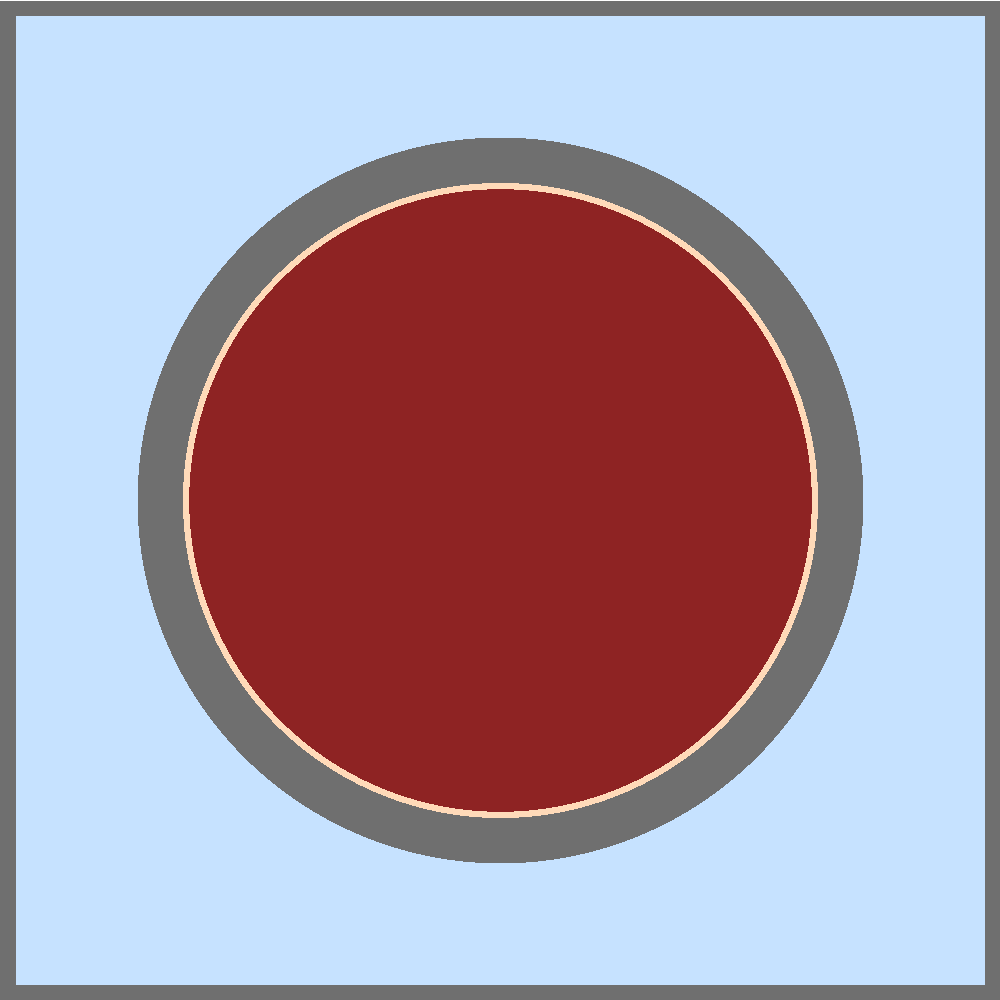
\includegraphics[width=0.9\linewidth]{figures/benchmarks/fuel-pin-16}
  \caption{}
  \label{fig:chap7-pin-1.6}
\end{subfigure}%
\begin{subfigure}{.5\textwidth}
  \centering
  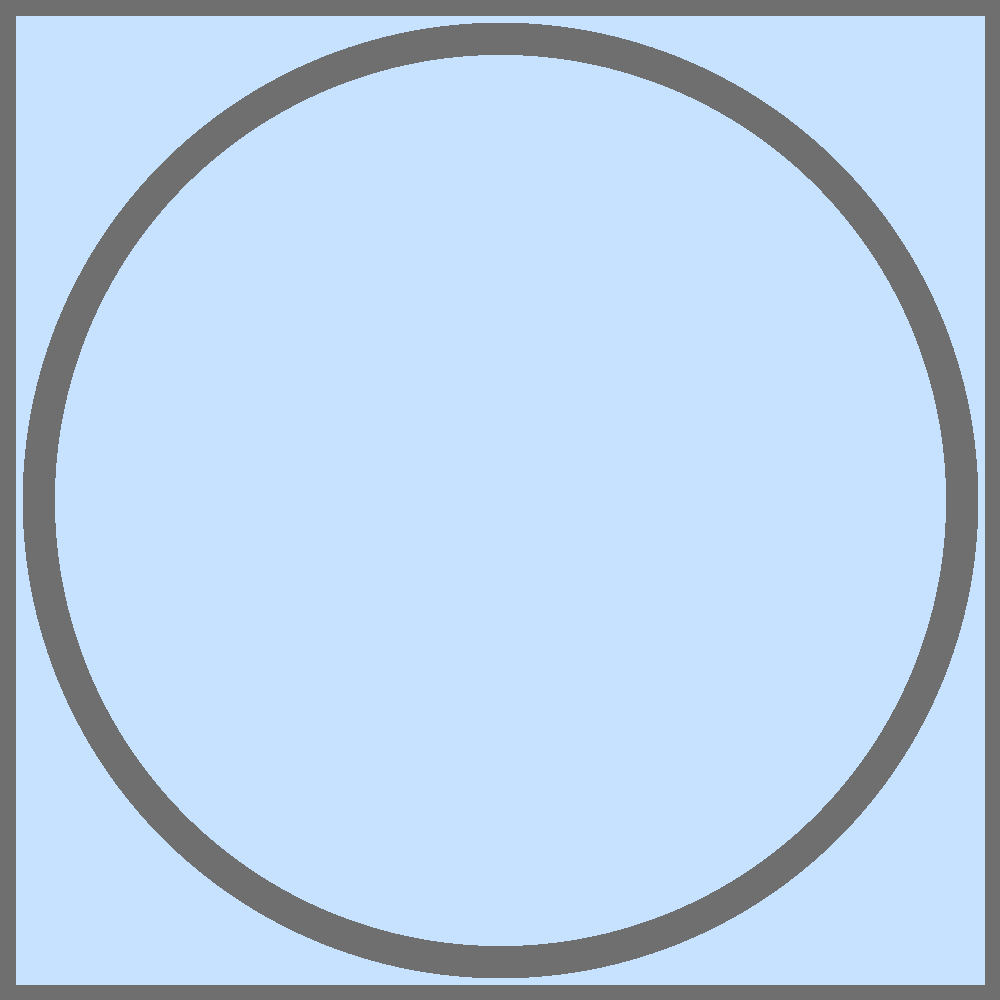
\includegraphics[width=0.9\linewidth]{figures/benchmarks/guide-tube}
  \caption{}
  \label{fig:chap7-pin-3.1}
\end{subfigure}
\begin{subfigure}{.5\textwidth}
  \centering
  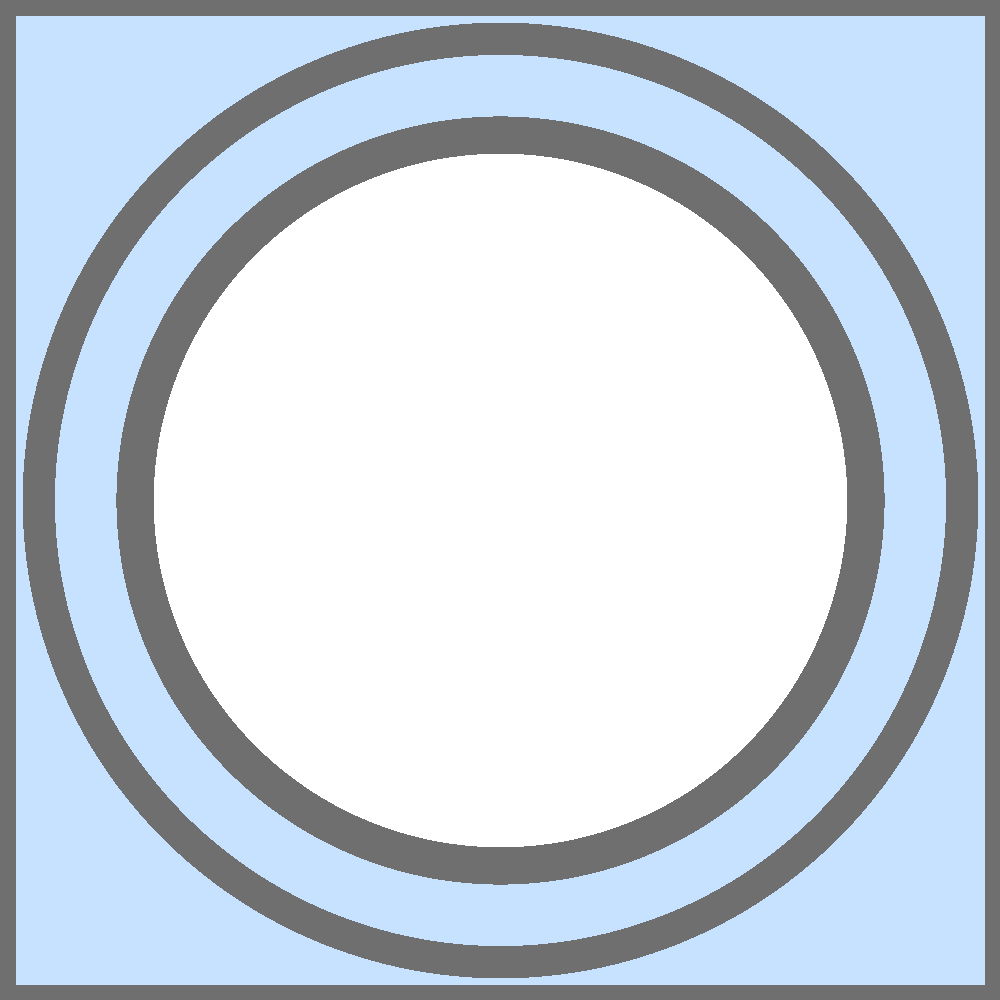
\includegraphics[width=0.9\linewidth]{figures/benchmarks/instr-tube}
  \caption{}
  \label{fig:chap7-guide-tube}
\end{subfigure}%
\begin{subfigure}{.5\textwidth}
  \centering
  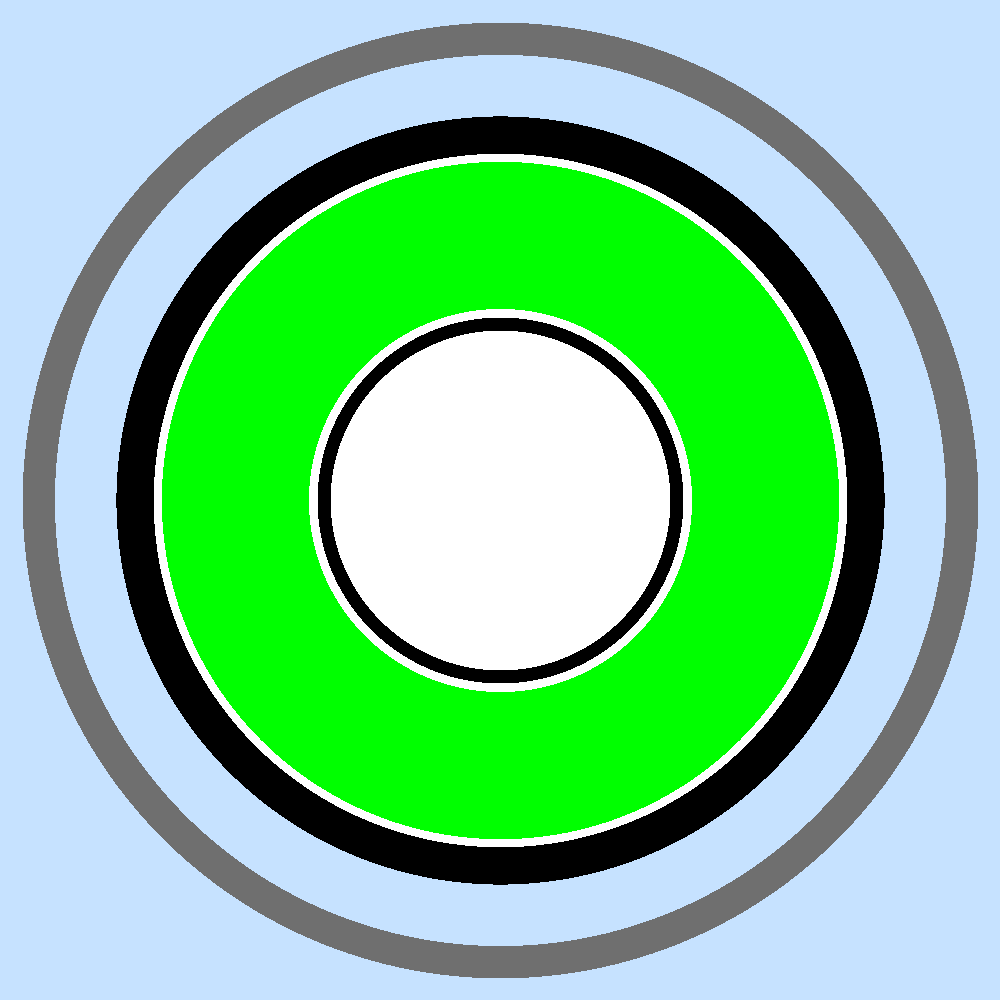
\includegraphics[width=0.9\linewidth]{figures/benchmarks/burn-abs}
  \caption{}
  \label{fig:chap7-instr-tube}
\end{subfigure}%
\caption[BEAVRS pin cell geometries]{1.6\% enriched fuel pin (a), control rod guide tube (b), instrument tube (c) and burnable absorber (d). Blue -- borated water, red -- UO$_2$ fuel, gray -- zircaloy, brown -- helium, white -- air, green -- borosolicate glass; black -- stainless steel.}
\label{fig:chap7-pin-cells}
\end{figure}

\begin{figure}[H]
\centering
\begin{subfigure}{\textwidth}
  \centering
  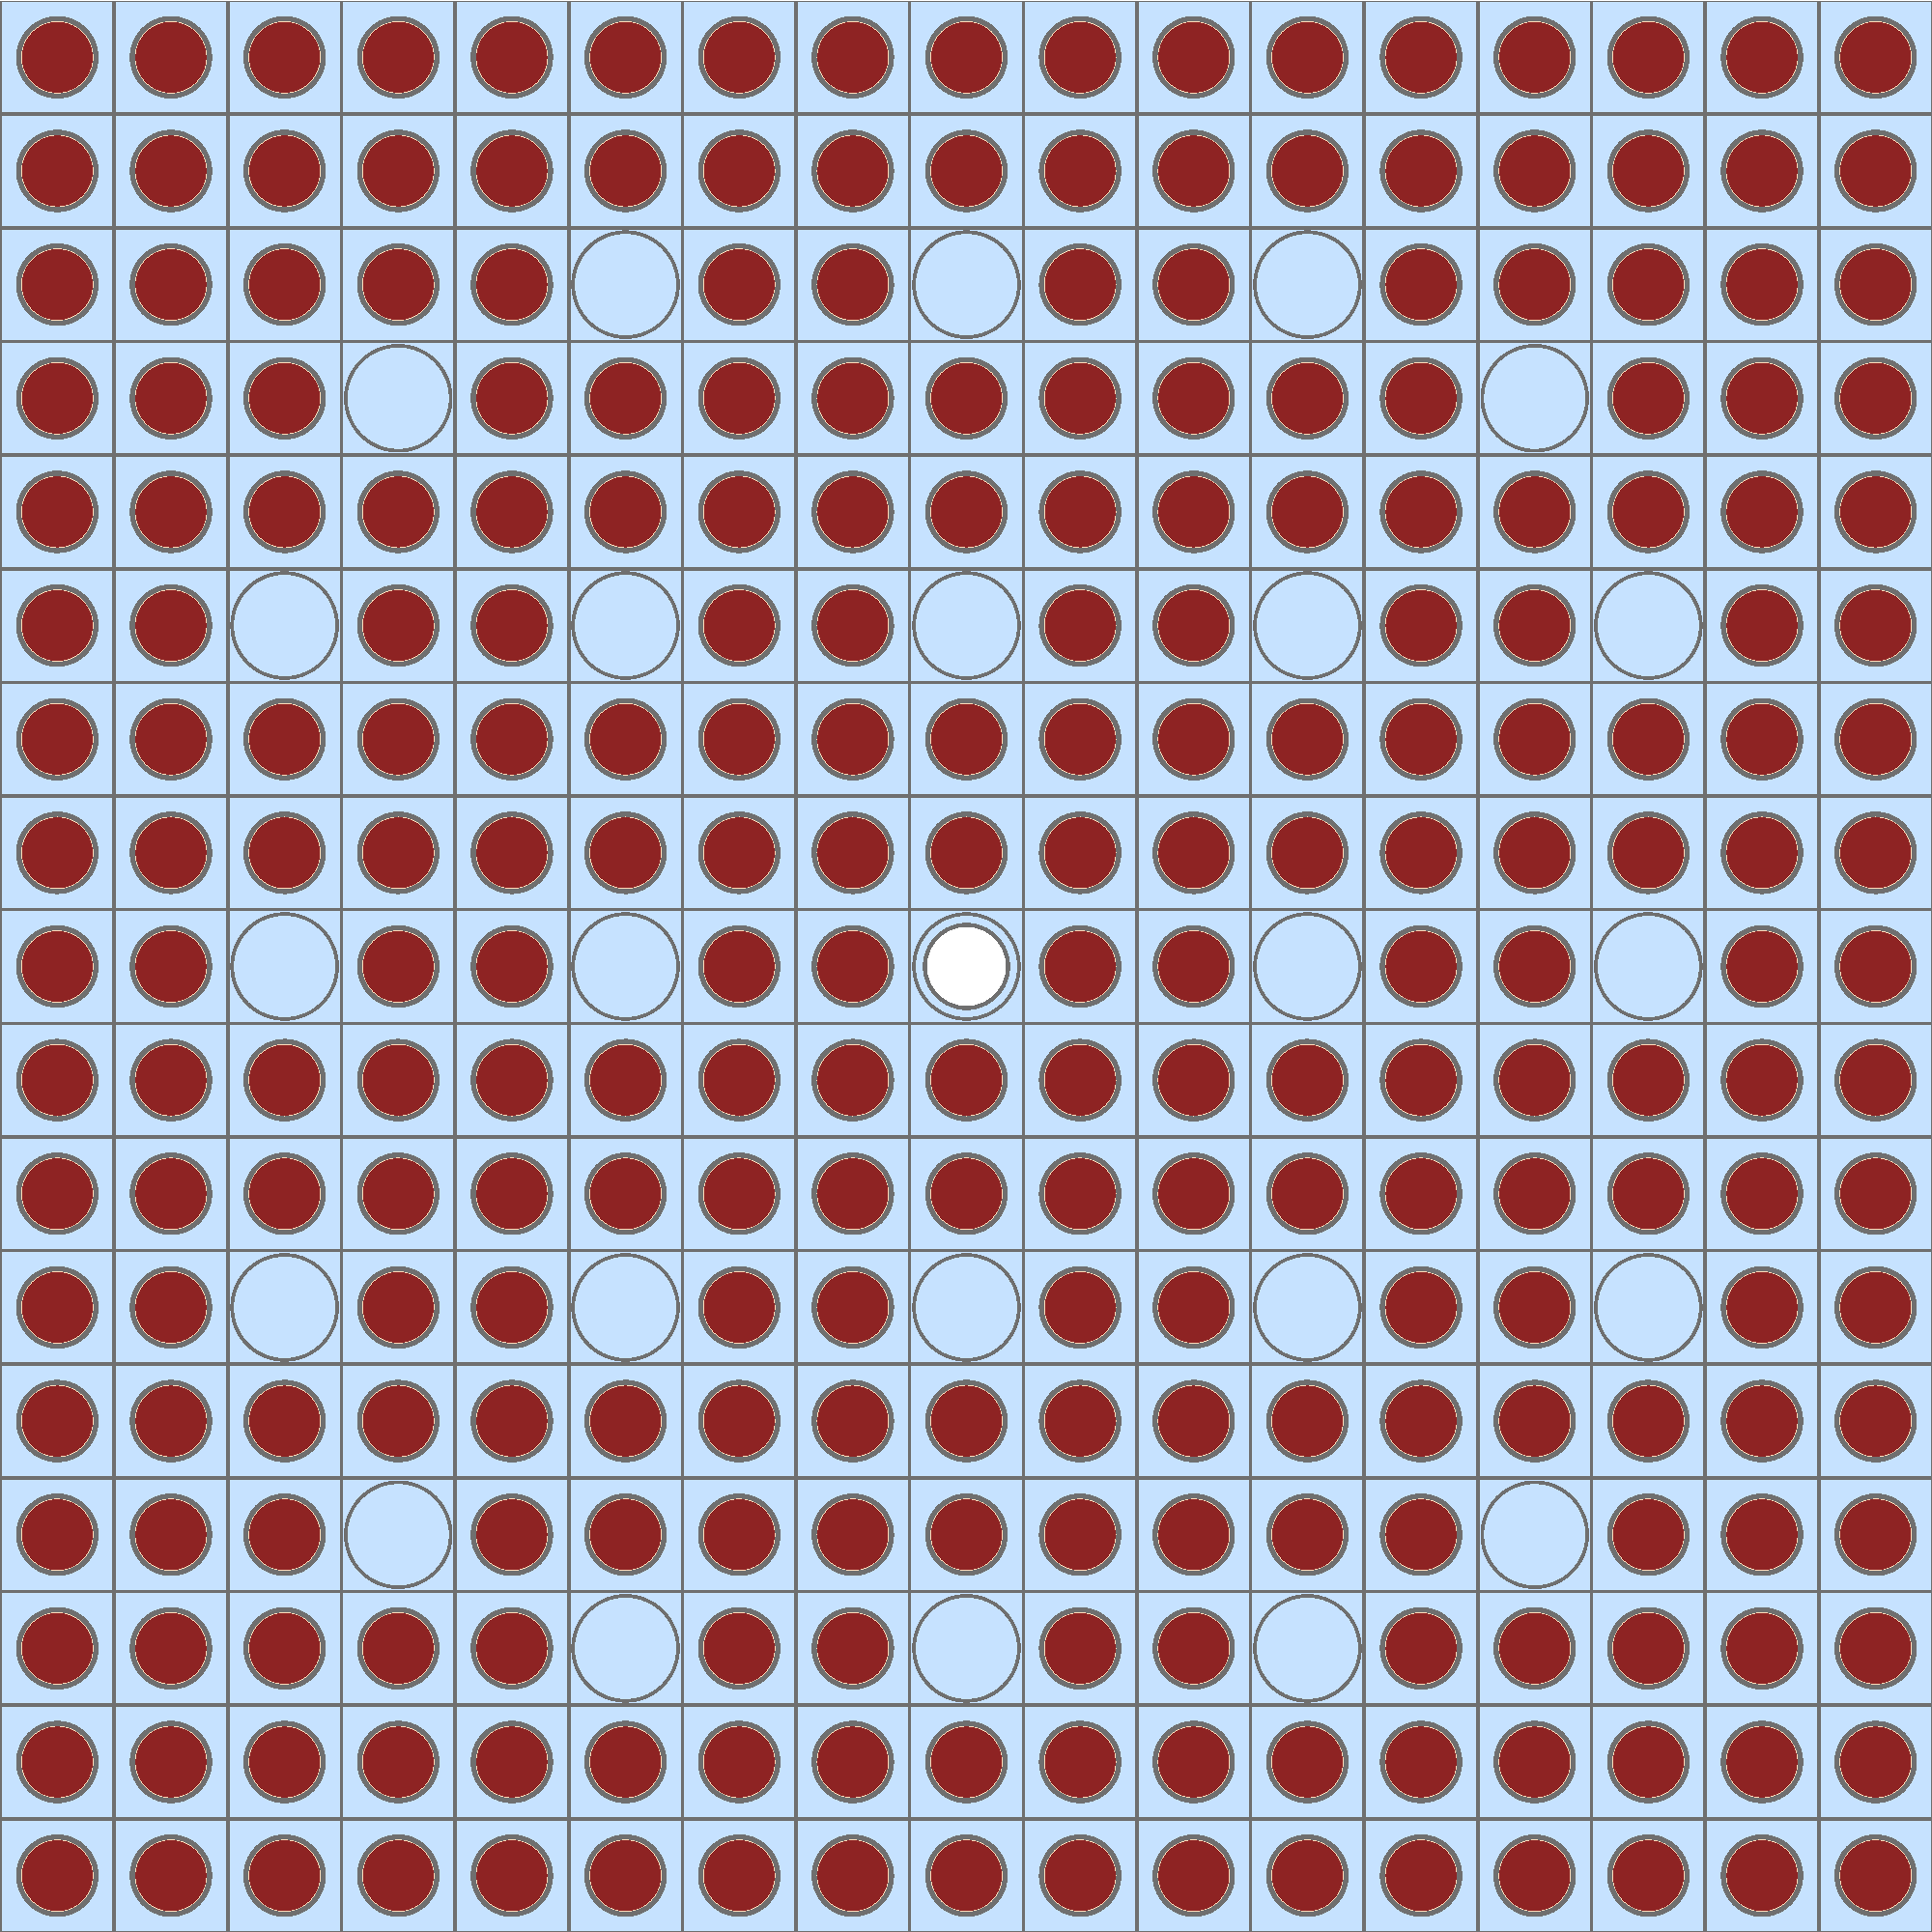
\includegraphics[width=0.4\linewidth]{figures/benchmarks/assembly-16}
  \caption{}
  \label{fig:chap7-assm-16}
\end{subfigure}
\begin{subfigure}{\textwidth}
  \centering
  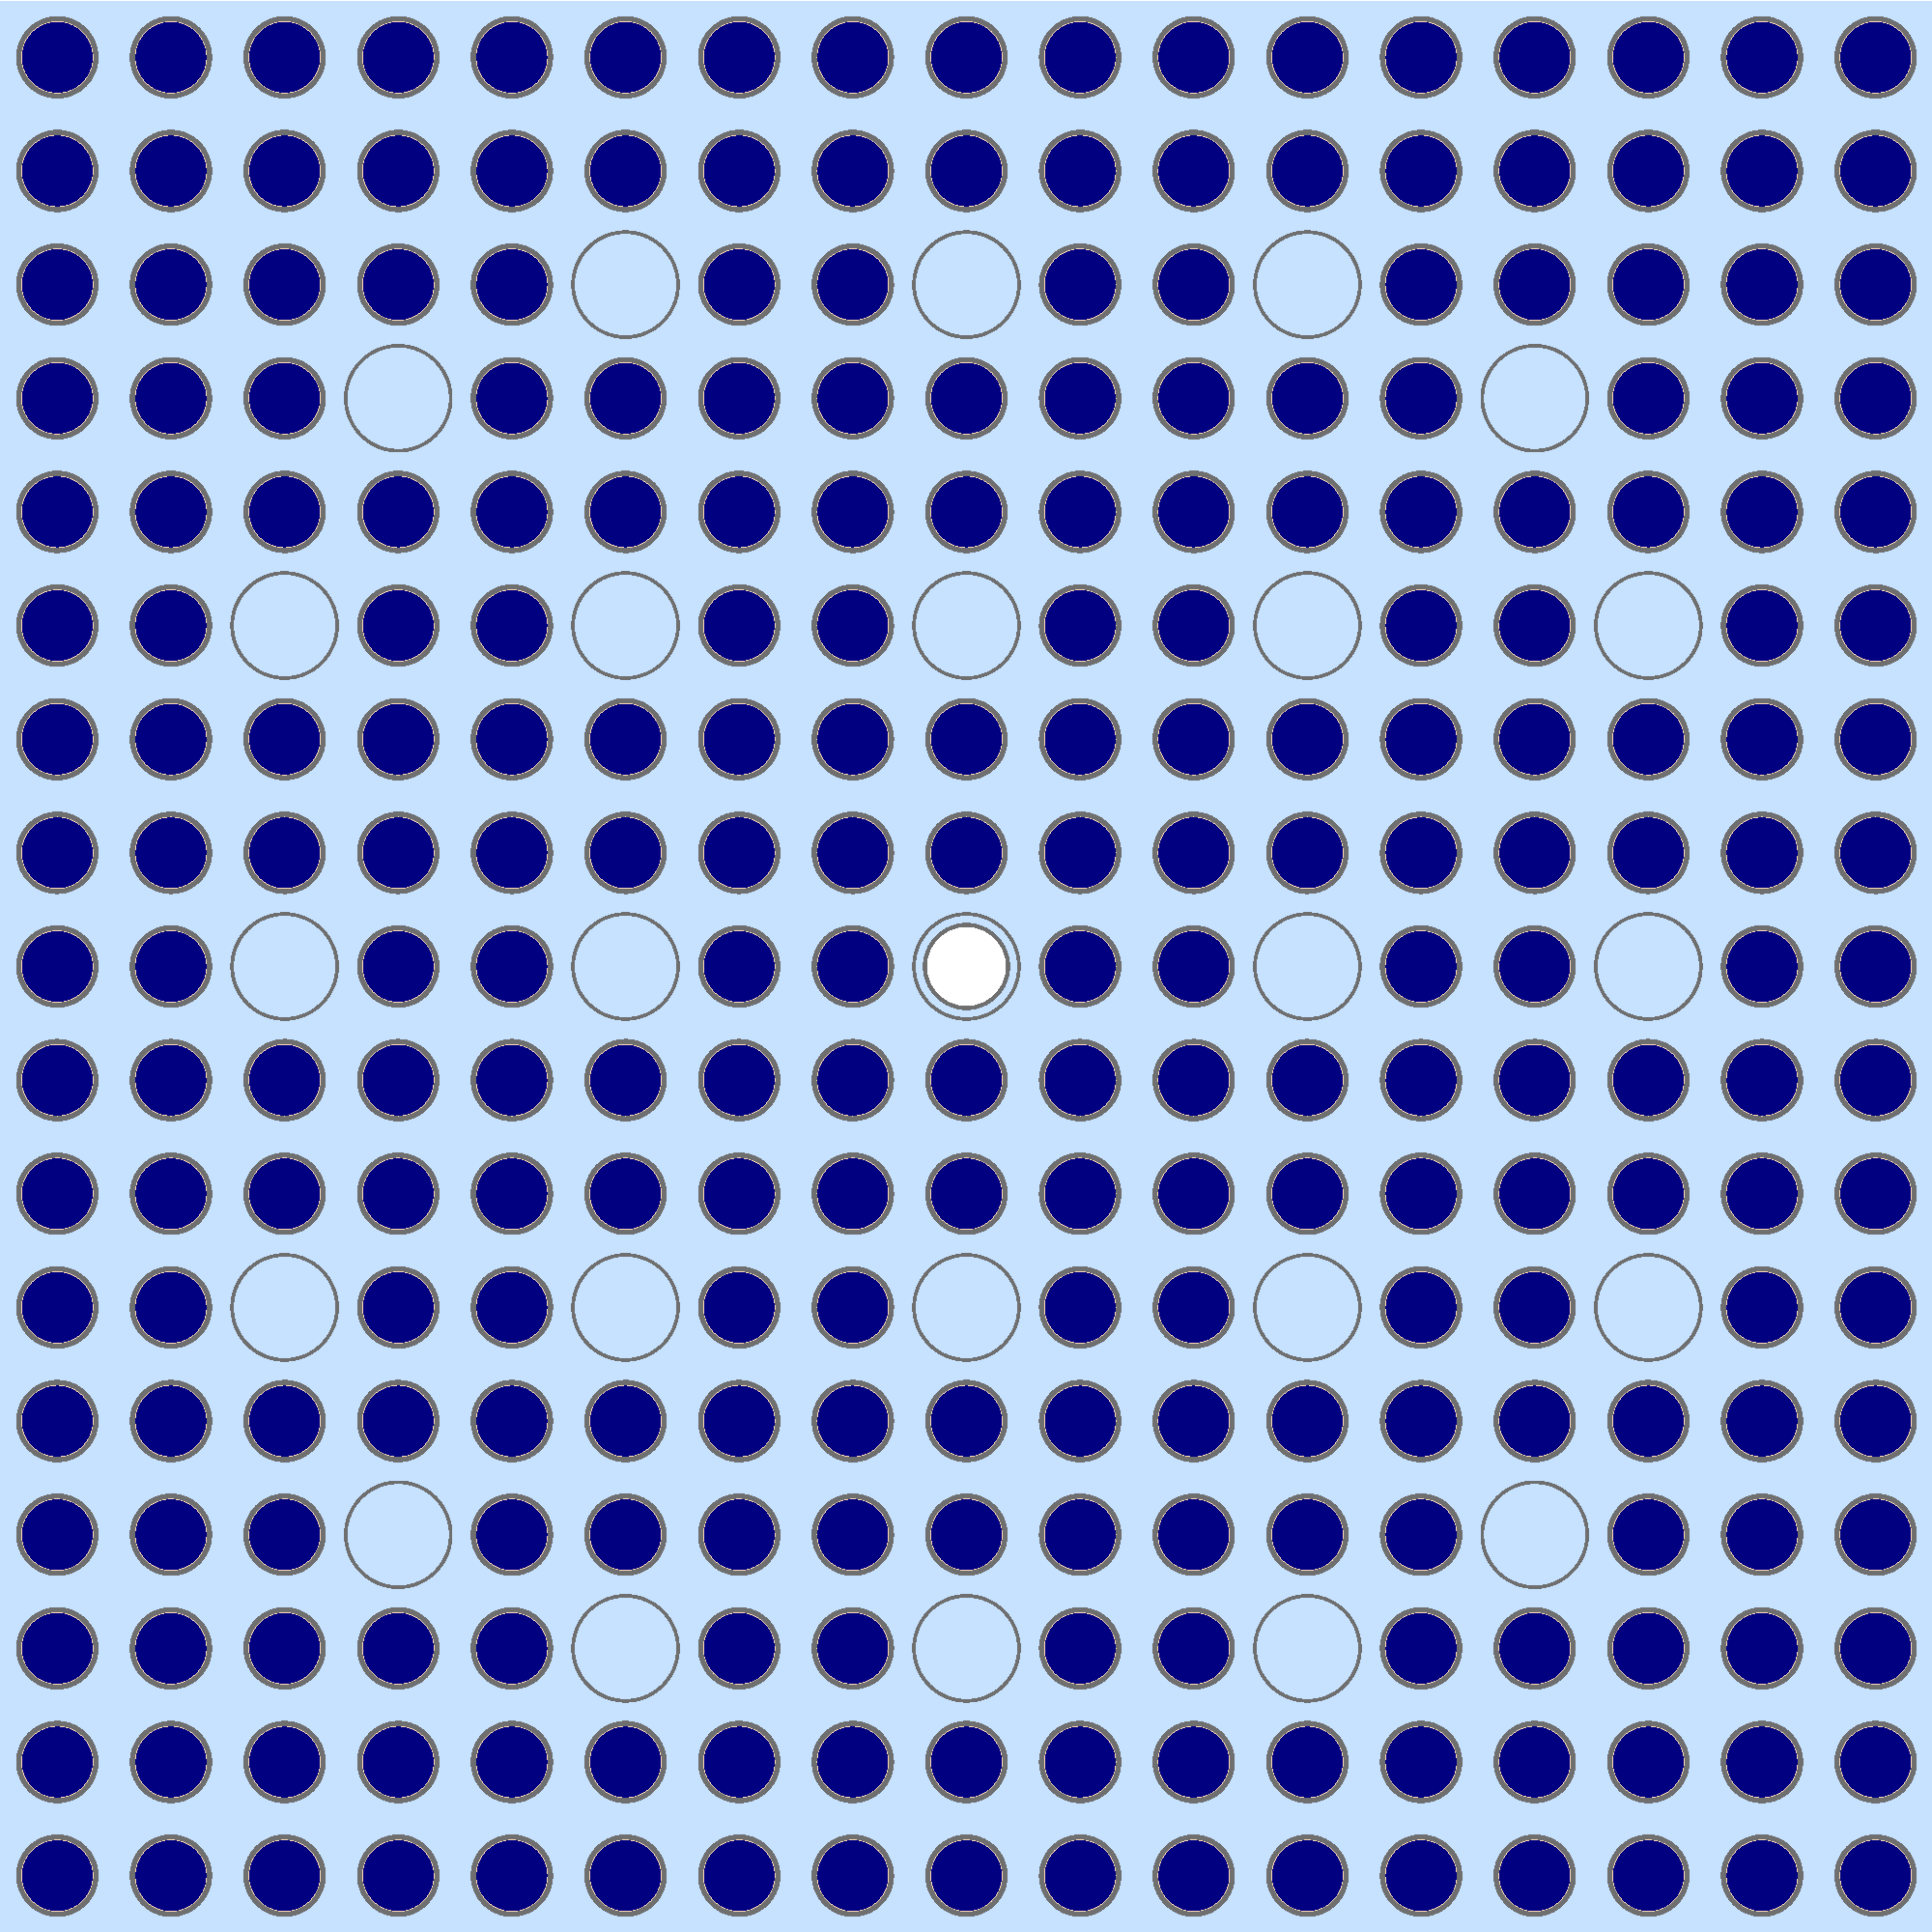
\includegraphics[width=0.4\linewidth]{figures/benchmarks/assembly-31}
  \caption{}
  \label{fig:chap7-assm-31}
\end{subfigure}
\begin{subfigure}{\textwidth}
  \centering
  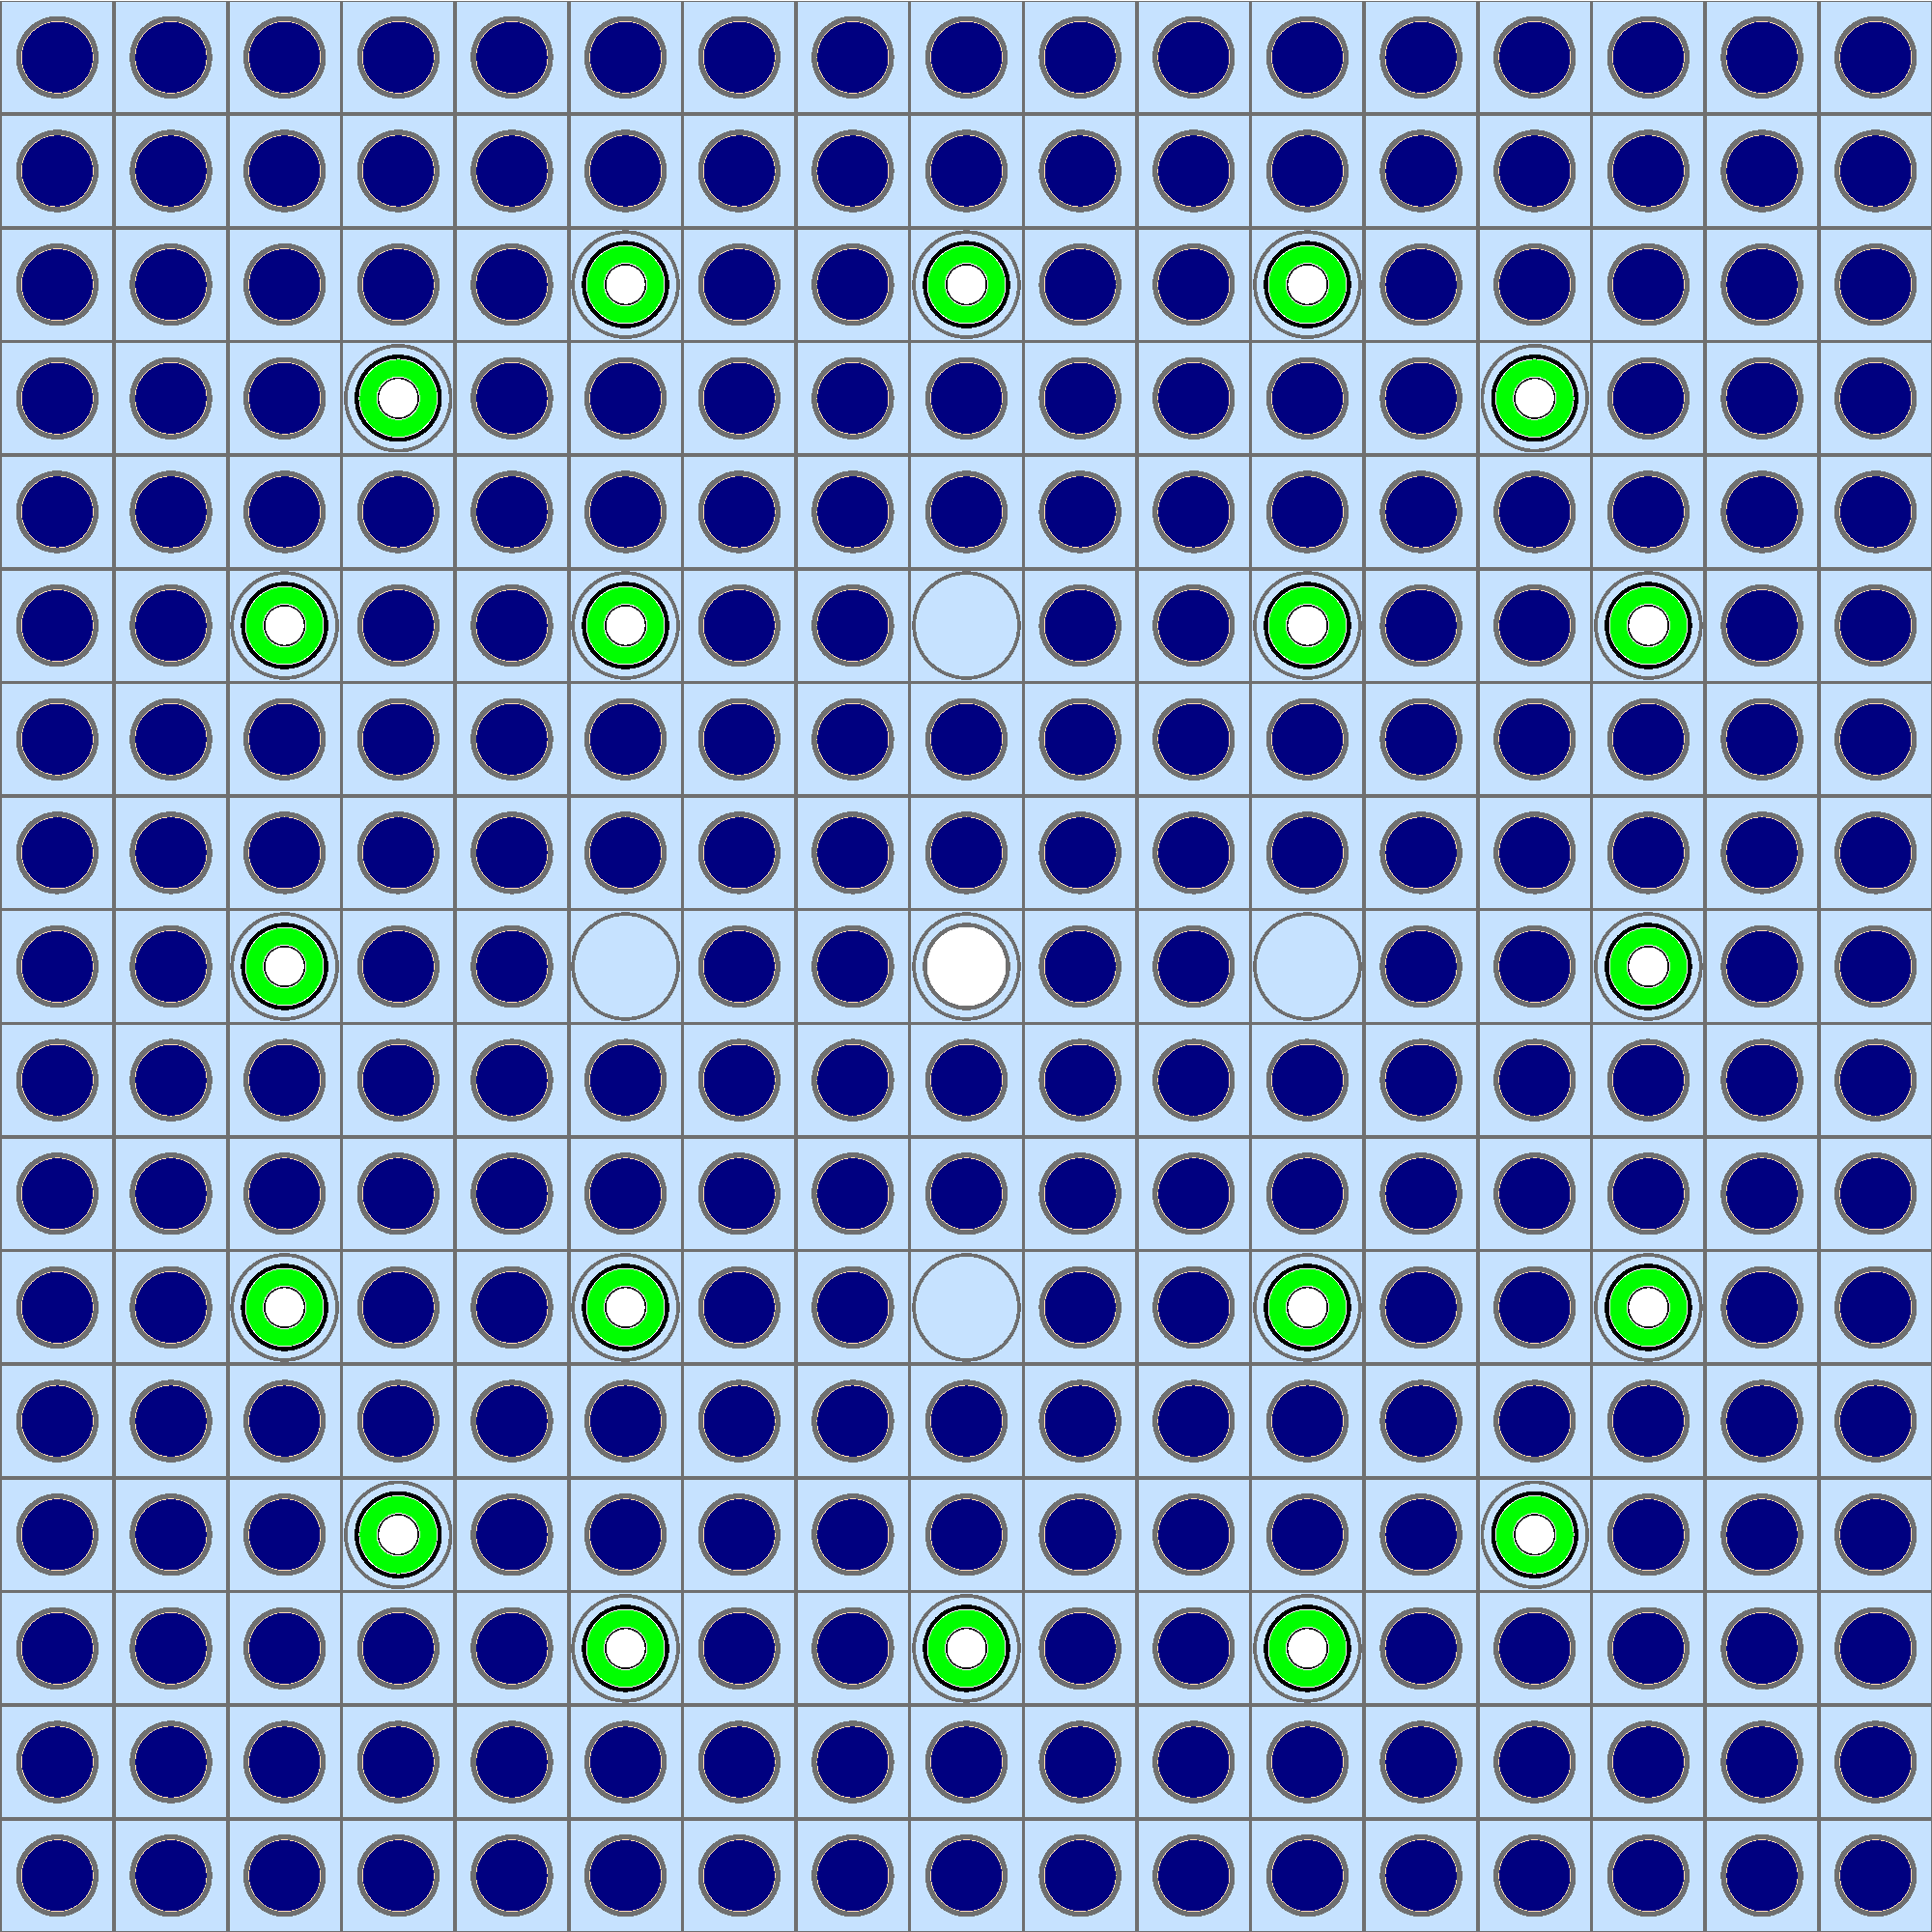
\includegraphics[width=0.4\linewidth]{figures/benchmarks/assembly-31-20BAs}
  \caption{}
  \label{fig:chap7-assm-31-20BAs}
\end{subfigure}%
\caption[BEAVRS fuel assembly geometries]{1.6\% enriched fuel pin (a), control rod guide tube (b), instrument tube (c) and burnable absorber (d). Blue -- borated water, red -- UO$_2$ fuel, gray -- zircaloy, brown -- helium, white -- air, green -- borosolicate glass; black -- stainless steel.}
\label{fig:chap7-fuel-assms}
\end{figure}

\begin{itemize}[noitemsep]
  \item geometric configuration
  \item isotopics
\end{itemize}

\subsection{Fuel Assemblies}

-figures of each type of sub-component in the geometry
-take from BEAVRS benchmark?

geometric specifications
-fuel pin, radii, clad, gap
-burnable poisons geometry above dashpot
-instrument tube

isotopics - take table format from Chap. 5 and specs from BEAVRS docs
-fuel
-water
-clad
-gap
-burnable absorber

\subsubsection{1.6\% Enriched Fuel}

-picture of geometry

\subsubsection{2.4\% Enriched Fuel}

-picture of geometry

\subsubsection{2.4\% Enriched Fuel with Burnable Absorbers}

-picture of geometry

\subsection{2$\times$2 Assembly Colorset}

-periodic BCs

\subsection{Reflector Geometry}

-add baffle to benchmark

\subsection{BEAVRS Full Core}


%%%%%%%%%%%%%%%%%%%%%%%%%%%%%%%%%%%%%%%%%%%%%%%%%%%%%%%%%%%%%%%%%%%%%%%%%%%%%%%
\section{Reference Results}

\subsection{Source Convergence}

-single plot of shannon entropy convergence by batch for each geometry

\subsection{Eigenvalues}

\begin{itemize}[noitemsep]
  \item converged values
  \item convergence by batch
\end{itemize}

\subsection{Pin Power Distributions}

\begin{itemize}[noitemsep]
  \item converged values
  \item convergence by batch
\end{itemize}

\subsection{U-238 Capture Rate Distributions}

\begin{itemize}[noitemsep]
  \item converged values
  \item convergence by batch
\end{itemize}


%%%%%%%%%%%%%%%%%%%%%%%%%%%%%%%%%%%%%%%%%%%%%%%%%%%%%%%%%%%%%%%%%%%%%%%%%%%%%%%
\section{Convergence Rates}

\begin{itemize}[noitemsep]
  \item quantify \# histories to $\pm$1 \ac{PCM}
  \item quantify \# histories to $\pm$1\% rel. err.
\end{itemize}